A Tabela \ref{results} apresenta os resultados  obtidos do grupo de teste contra o modelo para os quadros modelos
escolhidos após o treinamento, também apresenta o resultado do \textit{cross validation} com 5 iterações de cruzamento (cv).
Observando os resultados adquiridos é notável que os valores para \textit{Linear Regression}  são muito superiores aos para os outro modelos, e que \textit{Ridge Regression} obteve resultados ligeiramente  melhores que o \textit{State Vector Regression} para ambos os kernels.

\begin{table}[!ht]
\centering
    \caption{Valores do treinamento}
    \label{results}
\begin{tabular}{c c c}
    Modelo & resultado & resultado em cross validation (cv=5) \\
    \hline
    Linear Regression & 0.62 & -0.23,  0.27,  0.85,  0.89,  -0.73 \\
    SVR (linear) & 0.01 & -0.76, -0.44,  0.016, -0.023, -1.45 \\
    Ridge & 0.61 & -0.18,  0.30, 0.86,  0.88, -0.76 \\
    SVR (rbf) & 0.01 & -0.76, -0.44,  0.016, -0.022, -1.45
\end{tabular}   
\fonte{Próprio autor}
\end{table}

Entretanto, o objetivo não era ver o ajuste de novos dados dentro do universo esperado, mas sim se os mesmo poderiam se previsto, para tanto foram utilizados os valores das trintas últimas semanas. O gráfico \ref{predict} apresenta os resultados para a predição, apesar do excelente \textit{score} obtido pelo  \textit{Linear Regression} o mesmo não foi capaz de prever com extrema confiança o valor do preço do combustível, ficando ligeiramente abaixo que os valores realmente praticados. Quanto ao demais modelos, estes apresentaram resultados pouco efetivos destoando muito do preço esperado.

Interessante notar que o SVR para o \textit{kernel} rbf apresenta um formato de curva muito parecido com o do preço esperado, porém o mesmo é muito sensível ao ruído apresentado no gráfico da imagem \ref{dataset-graph}, logo, o seu resultado não condiz com o esperado.


\begin{figure}[!ht]
\centering
\caption{Gráfico do valores do \textit{dataset} e dos obtidos por \textit{Linear Regression} e \textit{Rigid Regression}}
\label{predict}
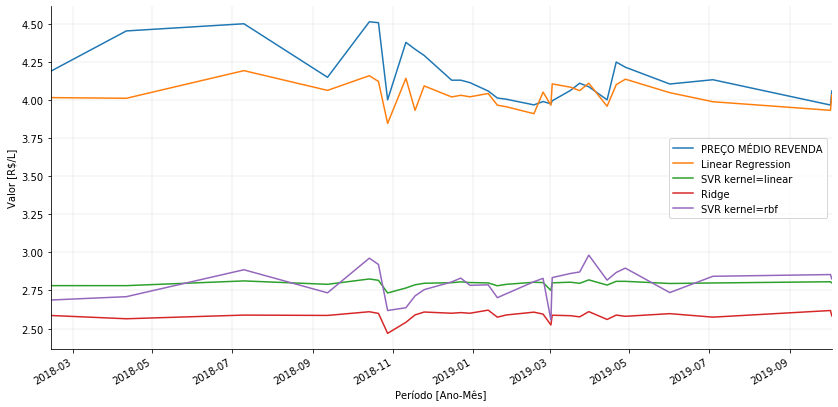
\includegraphics[width=1 \textwidth]{Figuras/predict.png}
\fonte{Próprio autor}
\end{figure}